\documentclass[paper]{IEEEtran}
\IEEEoverridecommandlockouts
% The preceding line is only needed to identify funding in the first footnote. If that is unneeded, please comment it out.
\usepackage[english]{babel}
\usepackage[utf8x]{inputenc}
\usepackage{amsmath}
\usepackage{graphicx}
\usepackage[colorinlistoftodos]{todonotes}
\usepackage{gensymb} % this could be problem
\usepackage{float}
\usepackage{fancyref}
\usepackage{subcaption}
\usepackage{amssymb}

\usepackage{pythonhighlight}

\usepackage{xspace}

\newcommand\nd{\textsuperscript{nd}\xspace}
\newcommand\rd{\textsuperscript{rd}\xspace}
\newcommand\nth{\textsuperscript{th}\xspace} %\th is taken already


\usepackage{xcolor}
\usepackage{listings}

\usepackage{fancyhdr}

\usepackage{karnaugh-map}

\definecolor{mGreen}{rgb}{0,0.6,0} % for python
\definecolor{mGray}{rgb}{0.5,0.5,0.5}
\definecolor{mPurple}{rgb}{0.58,0,0.82}


\definecolor{mygreen}{RGB}{28,172,0} % color values Red, Green, Blue for matlab
\definecolor{mylilas}{RGB}{170,55,241}

\lstdefinestyle{CStyle}{
    commentstyle=\color{mGreen},
    keywordstyle=\color{magenta},
    numberstyle=\tiny\color{mGray},
    stringstyle=\color{mPurple},
    basicstyle=\footnotesize,
    breakatwhitespace=false,         
    breaklines=true,                 
    captionpos=b,                    
    keepspaces=true,                 
    numbers=left,                    
    numbersep=5pt,                  
    showspaces=false,                
    showstringspaces=false,
    showtabs=false,                  
    tabsize=2,
    language=C
}


\lstset{language=Matlab,%
    %basicstyle=\color{red},
    breaklines=true,%
    morekeywords={matlab2tikz},
    keywordstyle=\color{blue},%
    morekeywords=[2]{1}, keywordstyle=[2]{\color{black}},
    identifierstyle=\color{black},%
    stringstyle=\color{mylilas},
    commentstyle=\color{mygreen},%
    showstringspaces=false,%without this there will be a symbol in the places where there is a space
    numbers=left,%
    numberstyle={\tiny \color{black}},% size of the numbers
    numbersep=9pt, % this defines how far the numbers are from the text
    emph=[1]{for,end,break},emphstyle=[1]\color{red}, %some words to emphasise
    %emph=[2]{word1,word2}, emphstyle=[2]{style},    
}



\makeatletter
\renewcommand\paragraph{\@startsection{paragraph}{4}{\z@}%
            {-2.5ex\@plus -1ex \@minus -.25ex}%
            {1.25ex \@plus .25ex}%
            {\normalfont\normalsize\bfseries}}
\makeatother
\setcounter{secnumdepth}{4} % how many sectioning levels to assign numbers to
\setcounter{tocdepth}{4}    % how many sectioning levels to show in ToC



\begin{document}

\title{EE314 Digital Electronics Laboratory\\
2017-2018 Spring Term Project Final Report\\
An FPGA Based Oscilloscope
}


\author{

\IEEEauthorblockN{1\textsuperscript{st} Halil TEMURTAS}
\IEEEauthorblockA{\textit{2094522} }
\textit{halil.temurtas@metu.edu.tr}

\and

\IEEEauthorblockN{2\textsuperscript{nd} Erdem TUNA}
\IEEEauthorblockA{\textit{2167419} }
\textit{erdem.tuna@metu.edu.tr}


}

\maketitle

\begin{abstract}

The design of an FPGA based digital oscilloscope 

\end{abstract}

\begin{IEEEkeywords}
FGPA, oscilloscope, ADC, VGA
\end{IEEEkeywords}

\section{Introduction}
\- \indent
	In this project, it is intended to realize a digital oscilloscope by using an FPGA. The FGPA will receive an analog signal, digitize it through an ADC; then will calculate the required parameters. Lastly data and input signal will be displayed on a VGA screen. The overall diagram is shown in \textit{Figure~\ref{fig:overall_diagram}}. The implementation logics and algorithms are discussed in respective sections.

\begin{figure}[h!]
	\setlength{\unitlength}{\textwidth}
	\center 
	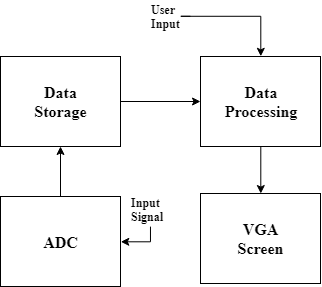
\includegraphics[width=0.47\textwidth]{overall_diagram}
	\caption{\label{fig:overall_diagram}The Block Diagram of the Project}
\end{figure}


\section{ALTERA DE1-SoC}
\- \indent
	In this project, we have used ALTERA DE1$\_$SoC Development Kit for main unit and a VGA Monitor as a screen for the oscilloscope. In this part, our aim is to introduce the FPGA used in the project. The overall look of the device can be seen at \textit{Figure~\ref{fig:FPGA}}, as can be seen from the figure, the Development Kit consists of multiple parts aside from FPGA. In this project, GPIO Pins, seven segment display, push buttons, switches and VGA output of DE1-SoC was used.  

\begin{figure}[H]
	\setlength{\unitlength}{\textwidth}
	\center 
	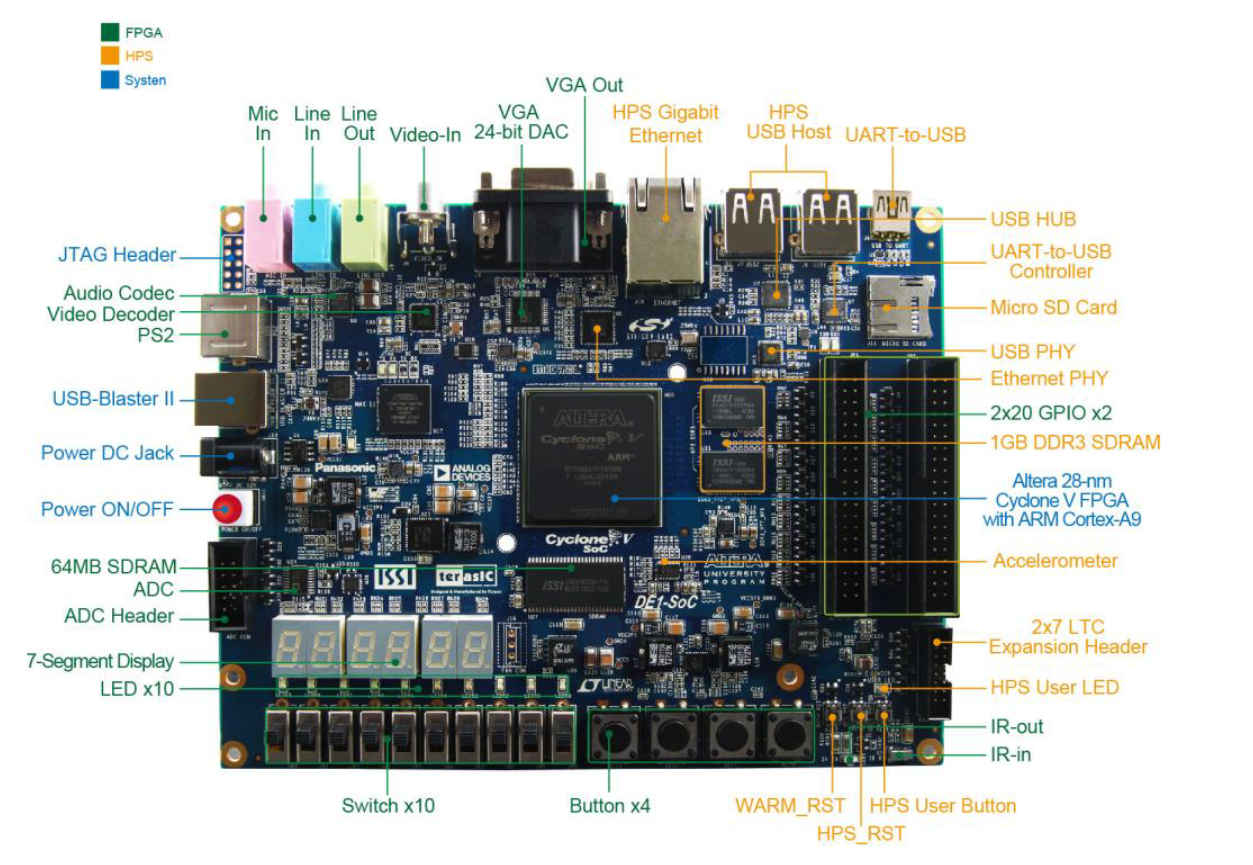
\includegraphics[width=0.47\textwidth]{FPGA}
	\caption{\label{fig:FPGA}ALTERA DE1$\_$SoC Development Kit}
\end{figure}

	GPIO pins, also known as general-purpose input/output pins, were used for getting the analog input that is desired to be monitored through oscilloscope. As can be seen from the \textit{Figure~\ref{fig:GPIO}}, the basic circuitry for this pins includes Schottky diodes for protection, and a resistor.
	
\begin{figure}[H]
	\setlength{\unitlength}{\textwidth}
	\center 
	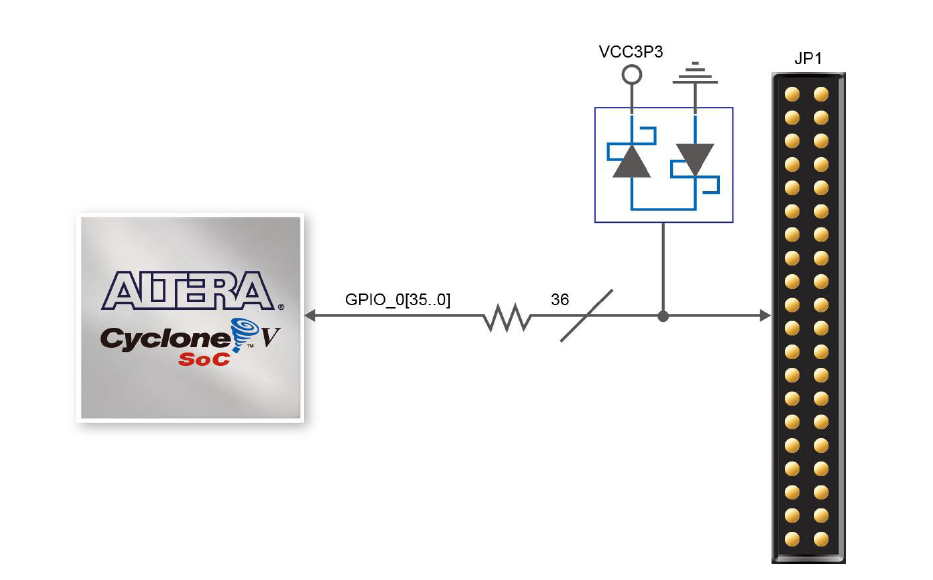
\includegraphics[width=0.47\textwidth]{GPIOpins}
	\caption{\label{fig:GPIO}GPIO Pins}
\end{figure}

	Seven segment display was used for testing the output values of computation value without using external monitor that we had some difficulties to find. As can be seen from the \textit{Figure~\ref{fig:SSD}}, every led on the seven segment is connected through a resistor to the FPGA.


\begin{figure}[H]
	\setlength{\unitlength}{\textwidth}
	\center 
	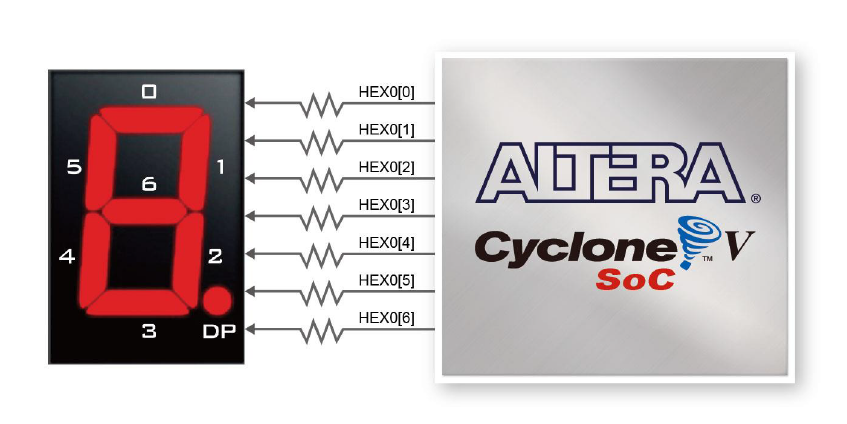
\includegraphics[width=0.47\textwidth]{SSD}
	\caption{\label{fig:SSD} Seven Segment Display}
\end{figure}

	Finally, the switch buttons were used as a mode buttons of the oscilloscope and push buttons were used as a division changer for the oscilloscope. The connections to FPGA can be seen at \textit{Figure~\ref{fig:pushbuttons}} and \textit{Figure~\ref{fig:switchbuttons}}. Finally the VGA connection used will be explained later in the report. 

\begin{figure}[h!]
	\setlength{\unitlength}{\textwidth}
	\center 
	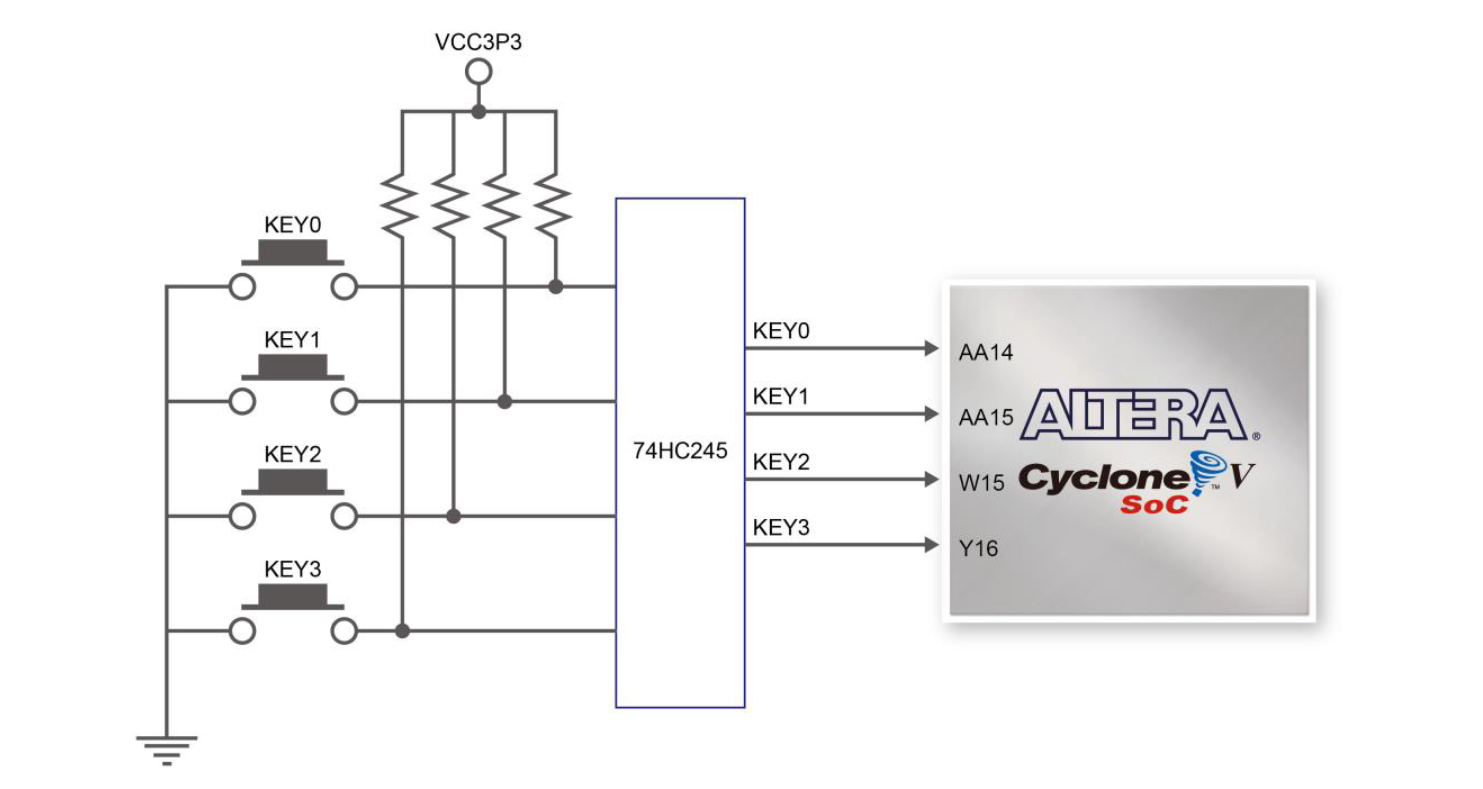
\includegraphics[width=0.47\textwidth]{pushbuttons}
	\caption{\label{fig:pushbuttons} Push Buttons}
\end{figure}


\begin{figure}[h!]
	\setlength{\unitlength}{\textwidth}
	\center 
	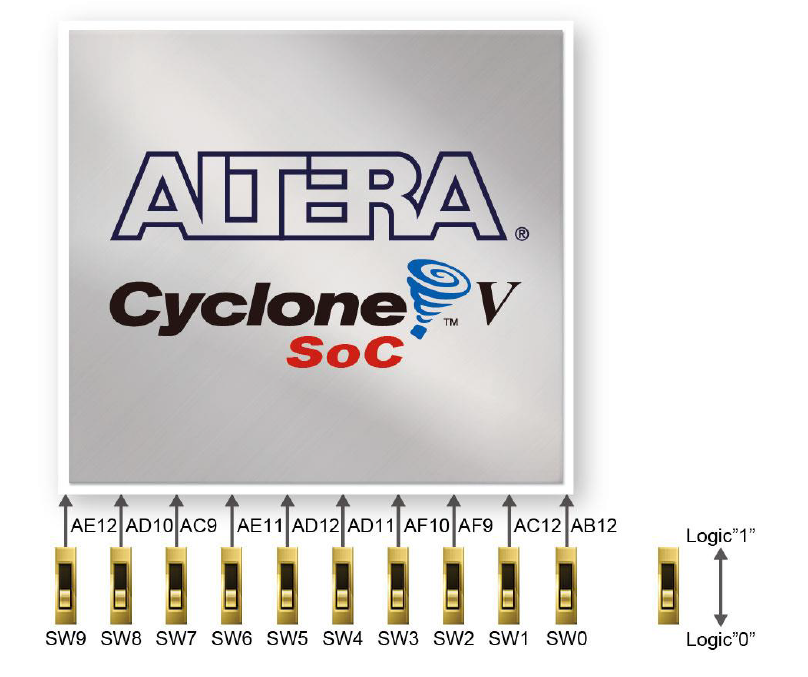
\includegraphics[width=0.47\textwidth]{switchbuttons}
	\caption{\label{fig:switchbuttons} Switch Buttons}
\end{figure}



\-\\[1cm]

\section{Modules}
\- \indent
	The modules and functional blocks designed and used in the project are presented in this section.
%\begin{figure}[h!]
%	\centering
%	\begin{subfigure}{.48\textwidth}
%		\centering
%		\includegraphics[width=1\linewidth]{scope_28_SimResult}
		%\caption{Theoretical Output of VCO.}
		%\label{fig:VCOFor1kHzTheoretical}
%	\end{subfigure}%
%	\newline
%	\begin{subfigure}{.48\textwidth}
%		\centering
%		\includegraphics[width=1\linewidth]{scope_28}
		%\caption{Practical Output of VCO.}
		%\label{fig:VCOFor1kHzPractical}
%	\end{subfigure}
	%\caption{VCO Outputs for 1kHz.}
%	\label{fig:VCOFor1kHz}
%\end{figure}

\subsection{ADC} \- \indent
		This module quantizes the analog input data. The hardware used is LTC2308 that is built into the FPGA. The Altera provides an example code regarding the use of the built-in ADC\cite{b1}. By evaluating the provided functionalities of this example with the help of a MsC project \cite{b2}, a code is written in Verilog HDL and in Qsys environment. Qsys instantiates the internal connections of embedded modules to use ADC controller. The resulting Qsys module is exported as BSF file and that is shown in \textit{Figure~\ref{fig:adc_block}}. This will be utilized as an ADC block. The code is written according to I/O ports of this block. But the ultimate ADC bus is output from "conduit\_end\_SDI" port of the ADC block. 
		
		\begin{figure}[H]
			\setlength{\unitlength}{\textwidth}
			\center 
			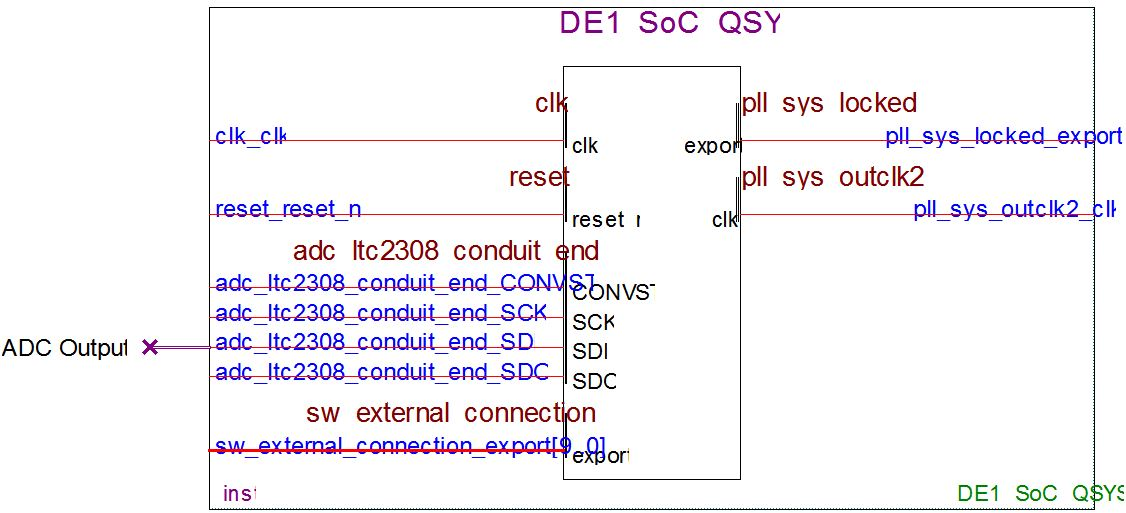
\includegraphics[width=0.47\textwidth]{adc_block}
			\caption{\label{fig:adc_block}The Block Diagram of the ADC}
		\end{figure}

\subsection{RAM} \- \indent
	The main function of RAM is to introduce a block to the system that can be both writable and readable. Writing is necessary to save data coming from ADC and reading is also necessary to process the data and show them on VGA screen. The RAM should work with FIFO structure to realize proper operation on VGA screen. "A FIFO (first-in-first-out) buffer is an "elastic" storage between two subsystems."\cite{b3}. A FIFO based read and write operation is depicted in \textit{Figure~\ref{fig:fifo_diagram}}. The RAM is designed in behaviour level however, yet not implemented. Possible state diagram for the RAM Module can be seen at \textit{Figure~\ref{fig:RAM State}}.
	
	\begin{figure}[t!]
		\setlength{\unitlength}{\textwidth}
		\center 
		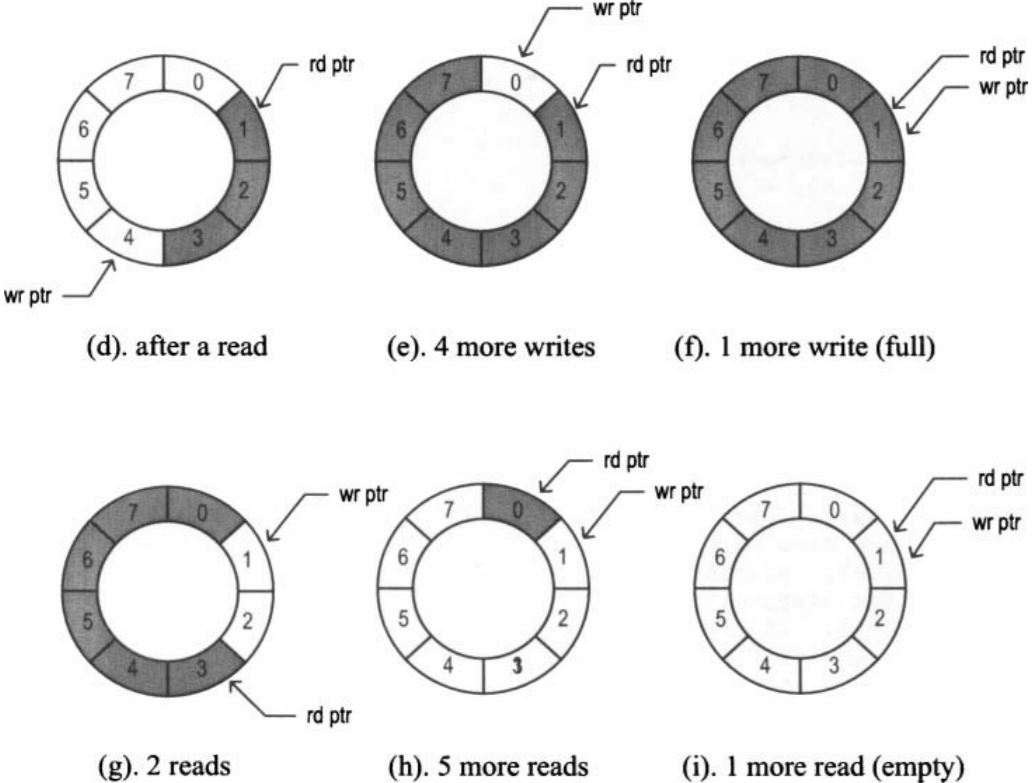
\includegraphics[width=0.47\textwidth]{fifo_diagram}
		\caption{\label{fig:fifo_diagram}FIFO Working Principle\cite{b3}}
	\end{figure}

\begin{figure}[h!]
			\setlength{\unitlength}{\textwidth}
			\center 
			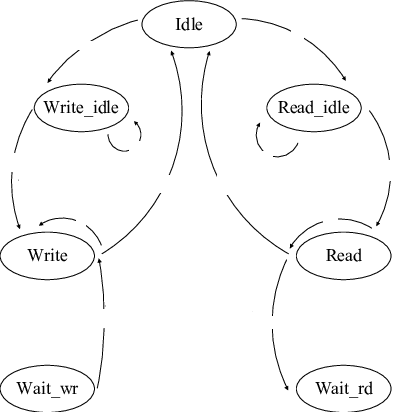
\includegraphics[width=0.47\textwidth]{RAM_state}
			\caption{\label{fig:RAM State} State Diagram for RAM}
\end{figure}
		
		
\subsection{Computation Unit} \- \indent
	Computation unit is the unit responsible for all kinds of mathematical calculation of the project. For instance mean value calculation for the input signal are conducted in this unit. This Unit can be considered as a brain of the project. Some important parts are as follows,	

\begin{figure}[h!]
	\setlength{\unitlength}{\textwidth}
	\center 
	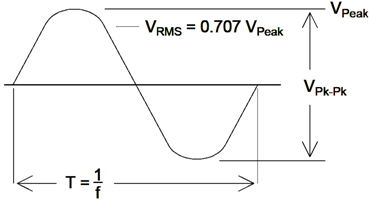
\includegraphics[width=0.47\textwidth]{voltage}
	\caption{\label{fig:waveform} Voltage Waveform and its Properties}
\end{figure}

\- \\[4cm]

\paragraph{Peak-to-Peak Value Calculation}	
\- \indent
	To find the peak-to-peak value of the input voltage, we needed to find the maximum and minimum voltage values of the given input. For that purpose we have used a well known sorting algorithm. Initially a point on the waveform was picked and every point next to it was compared to it. If the next point on the voltage is bigger than the initially stored value, the stored value is replaced with that value. After tracing every point on the waveform, the biggest value can be found. Similarly, the lowest value on the voltage waveform can be found. 
	
	After finding minimum and maximum points at the voltage waveform, peak-to-peak value is the difference between these values as can be seen from the \textit{Figure~\ref{fig:waveform}}.  	
	
	
\paragraph{Mean Value Calculation}


\paragraph{DC Offset Calculation}

DC offset is a mean amplitude displacement from


\paragraph{Frequency Calculation}



\subsection{Mode Selection (AC/DC)} \- \indent
	AC/DC Modes are one of the most fundamental mods of digital oscilloscopes in market. In this part we will build a module to build our own selection mode. One slide switch will be assigned to retrieve the desired mode information from the user. Based on this information, screen will display the input signal either with the DC offset or without the DC offset.

\subsubsection{AC Mode} \- \indent
	In AC Mode operation of the oscilloscope, the DC offset voltage is removed from the input voltage before it is reflected to the VGA monitor. For that Computation Unit will be used to extract offset information from stored data.

\subsubsection{DC Mode} \- \indent
	In DC Mode operation of the oscilloscope, the DC offset voltage is untouched from the stored data of the input voltage. The stored data is reflected directly to the VGA monitor. 
	

\subsection{VGA Screen} \- \indent
	VGA is a widely used standard in video industry for the transmission of video signals from a computer or microprocessor into a monitor or TV. The input pin configuration for the VGA Monitor can be seen at \textit{Figure~\ref{fig:vga_pins}}. VGA provides 640x480 pixel resolution. This resolution, however, is not the total pixel in horizontal and vertical axes. There is a blank border frame surrounding the display area. The horizontal axis has 48 pixels of border width on the left and 16 pixels of border width on the right side of the screen. Additionally, there are 96 pixels of border width for ray tube the retrace through the diagonal of the screen. The vertical axis has also similar additional pixels. 10 and 33 pixels for top and bottom borders, respectively. Also 2 pixels for the vertical retrace of the ray tube. The total structure of a VGA screen can be seen in \textit{Figure~\ref{fig:vga-hsync-vsync}}. The whole screen is 800x525 pixels.
	
\begin{figure}[h!]
			\setlength{\unitlength}{\textwidth}
			\center 
			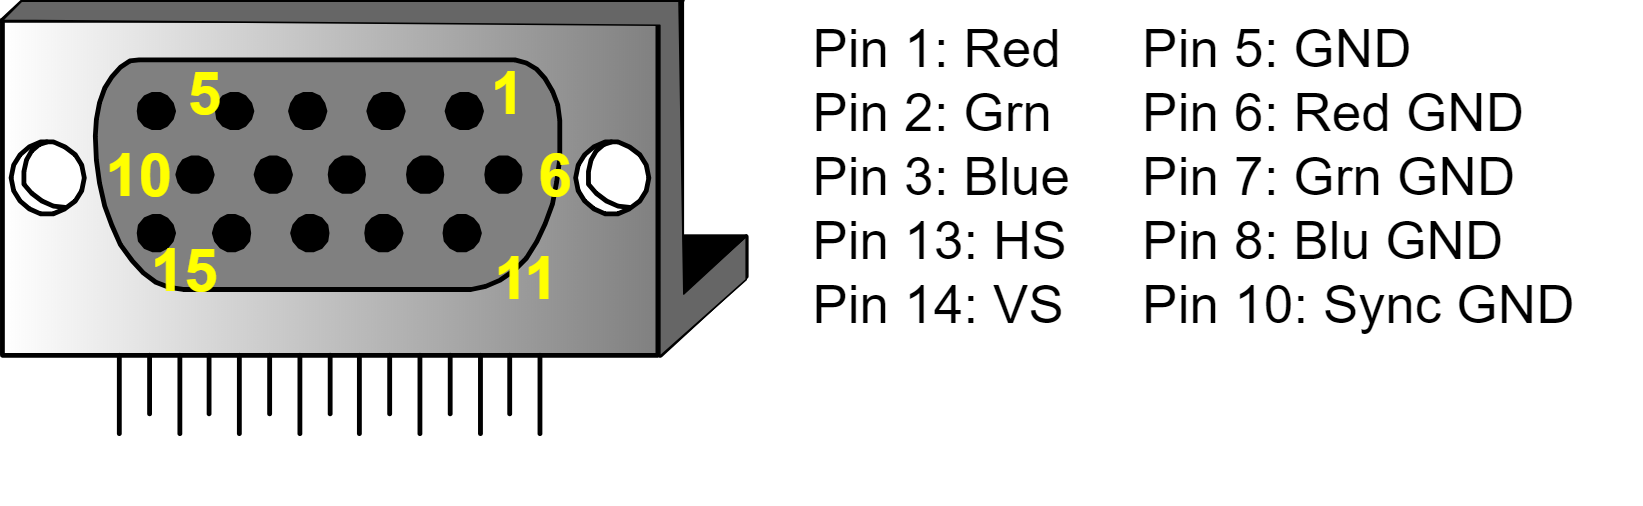
\includegraphics[width=0.47\textwidth]{vgapins}
			\caption{\label{fig:vga_pins} VGA Input Pins}
\end{figure}


\begin{figure}[h!]
	\setlength{\unitlength}{\textwidth}
	\center 
	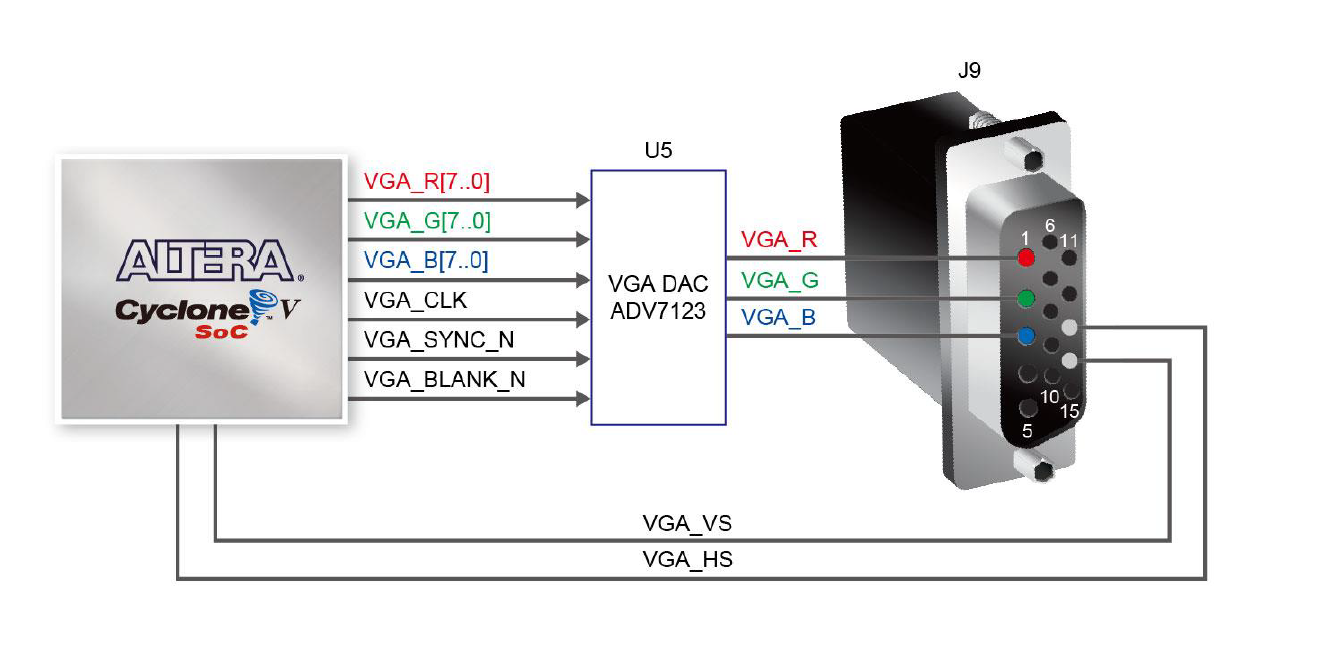
\includegraphics[width=0.47\textwidth]{VGAconfig}
	\caption{\label{fig:VGA_config}The Block Diagram of the Project}
\end{figure}

\begin{figure}[h!]
	\setlength{\unitlength}{\textwidth}
	\center 
	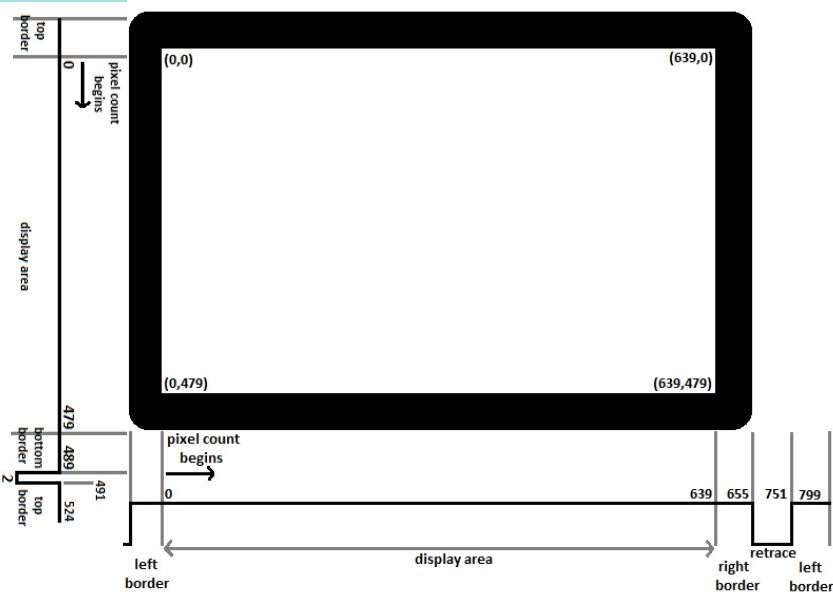
\includegraphics[width=0.47\textwidth]{vga-hsync-vsync}
	\caption{\label{fig:vga-hsync-vsync}The Block Diagram of the Project}
\end{figure}

\subsubsection{VGA Controller} \- \indent

	The VGA controller combines the data from RAM and Computation Unit to create a signal that can be displayed on the VGA monitor. Each of the RAM Modules contains an image that is ready for display on the screen. However, the data must be positioned relative to each other and combined. Also this module performs once a second as desired in the project requirements. The VGA controller also gets data from different data inputs such as Time/div and Voltage/div in order to reflect the waveform as user requires. In this part multiple clock signals and counters needed to display the waveform accordingly. Basic VGA Controller can be seen at \textit{Figure~\ref{fig:vga_controller}}\cite{b4}.

\begin{figure}[h!]
			\setlength{\unitlength}{\textwidth}
			\center 
			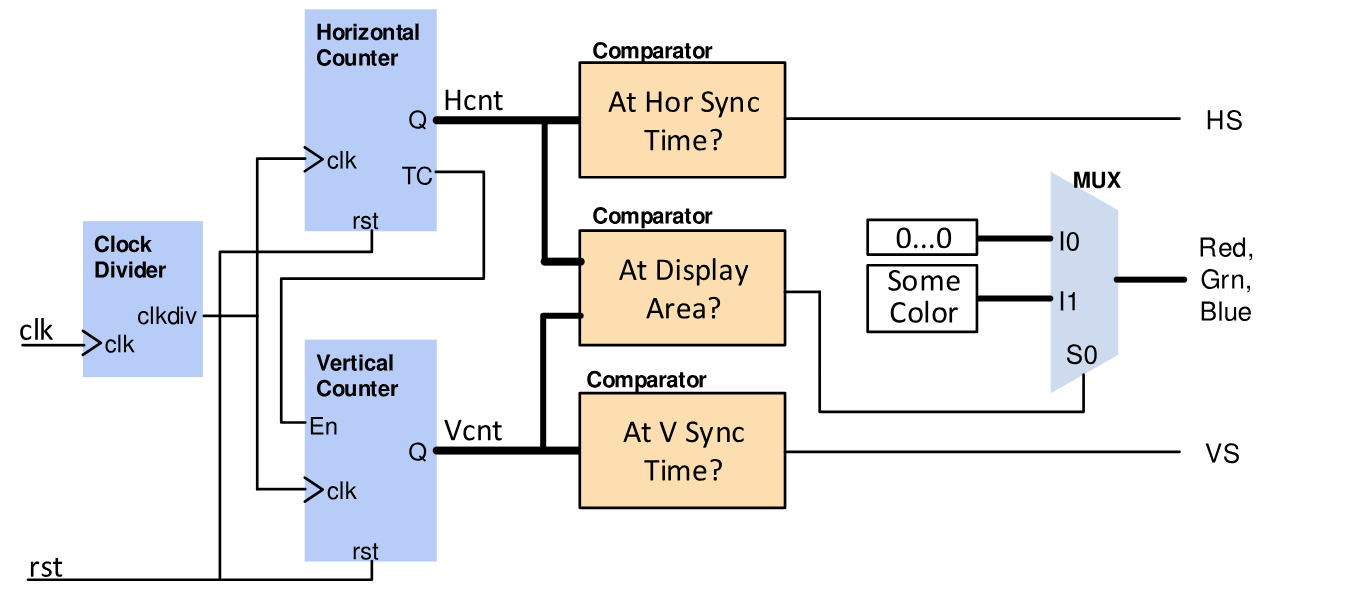
\includegraphics[width=0.47\textwidth]{vgacontroller}
			\caption{\label{fig:vga_controller} VGA Controller}
\end{figure}
		
			
	This module will supply an input data for the VGA controller for user preferences. Two push buttons will be assigned for the Time/div inputs that can be considered as Time+/div and Time-/div. As user pushes to Time+/div button, the time scale will be larger than the previous value. Similarly, as the user pushes to Time-/div button, the time scale will be smaller than the previous value. According to user preferences, this module allows user to see wider or narrower parts of input waveform.

\vfill	 
	  
\subsubsection{Voltage/div Input} \- \indent

	This module will supply an input data for the VGA controller for user preferences. Two push buttons will be assigned for the Voltage/div inputs that can be considered as Voltage+/div and Voltage-/div. As user pushes to Voltage+/div button, the voltage scale will be larger than the previous value. Similarly, as the user pushes to Voltage-/div button, the voltage scale will be smaller than the previous value. According to user preferences, this module allows user to fit the voltage waveform to the screen.
	
\subsubsection{Autoscale Input} \- \indent

	This module will also supply an input data for the VGA controller for user preferences. Since we are planning to use all push buttons for other modules. One slide switch will be assigned to this module. As the user triggers the button, this module will scale the waveform for the display such that it fits the display best.

	
	
\section{Conclusion}
\- \indent
	In this project, our aim is to design a FPGA based digital oscilloscope using Verilog. The project consists of five main part that are Analog to Digital Converter (VGA), RAM, Computation Unit, Mode Selection for Display and VGA Screen. Overall diagram of the project can be seen at \textit{Figure~\ref{fig:overall_diagram}}. 
	
	

\begin{thebibliography}{00}
\bibitem{b1} “De1-Soc CD.” [Online]. Available: http://download.terasic.com/downloads/cd-rom/de1-soc/DE1-SoC\_v.5.0.1\_HWrevF\_SystemCD.zip. [Accessed: 21-May-2018].
\bibitem{b2} “Digital Scope Implemented on Altera DE1-SoC.” [Online]. Available: https://people.ece.cornell.edu/land/courses/eceprojectsland/STUDENTPROJ/\\2015to2016/hj424/hj424\_report\_201605191237.pdf. [Accessed: 21-May-2018].
\bibitem{b3} P.P. Chu, Embedded SoPC Design with NIOS II Processor and Verilog Examples. New Jersey, 2012.
%\bibitem{b3} “2N7000 Datasheet.” [Online]. Available: https://www.onsemi.com/pub/Collateral/2N7000-D.PDF. [Accessed: 20-Jan-2018].
\bibitem{b4} "VGA Display Controller" [Online]. Avaible : https://learn.digilentinc.com/Documents/269
%\bibitem{b6} Y. Yorozu, M. Hirano, K. Oka, and Y. Tagawa, ``Electron spectroscopy studies on magneto-optical media and plastic substrate interface,'' IEEE Transl. J. Magn. Japan, vol. 2, pp. 740--741, August 1987 [Digests 9th Annual Conf. Magnetics Japan, p. 301, 1982].
%\bibitem{b7} M. Young, The Technical Writer's Handbook. Mill Valley, CA: University Science, 1989.
\end{thebibliography}




\end{document}